\section{Independent pressure--speciation--calorimetry comparison}

\subsection{Question and method}

Does the small loss in former-reserved speciation accuracy outweigh the pressure and
calorimetry improvements from the calorimetry-balanced reaction-temperature
candidate? The comparison uses frozen evidence outside the parameter fit, but
not an untouched independent-validation partition: 27 temperature-challenge
pressure rows, 67 former-reserved speciation targets, and 69
direct 30 wt\% MEA calorimetry observations. The exact nonlinear candidate
replay evaluated all 70 pressure/speciation states without failure.

Errors have different units, and complete observation covariance is not
available. Each domain error is therefore normalized by the retained-set error.
For nonnegative domain weights $w_d$ summing to one, the comparison score is

\[
S=\prod_d\left(\frac{E_{d,\mathrm{balanced}}}
{E_{d,\mathrm{retained}}}\right)^{w_d}.
\]

A score below one favors the calorimetry-balanced set. The weights represent
engineering priorities rather than measurement-uncertainty weights.

\subsection{Result}

\begin{table}[htbp]
\centering
\caption{Multiproperty errors and balanced-to-retained ratios.}
\begin{tabular}{lrrr}
\toprule
Domain & Retained & Balanced & Ratio \\
\midrule
Pressure ln-RMSE & 0.7932 & 0.7133 & 0.899 \\
Reserved-speciation ln-RMSE & 0.8481 & 0.8830 & 1.041 \\
Calorimetry RMSE (kJ/mol CO$_2$) & 15.755 & 10.489 & 0.666 \\
\bottomrule
\end{tabular}
\end{table}

Equal domain weighting gives $S=0.854$, a 14.6\% reduction in combined
normalized error. A 0.01-spaced sweep of all 5151 nonnegative weight
combinations favors the balanced set for 97.2\% of the grid. The retained set
is selected only when reserved speciation receives more than 72.5--91.0\% of
the total weight; the threshold depends on the pressure/calorimetry split.

\begin{figure}[htbp]
\centering
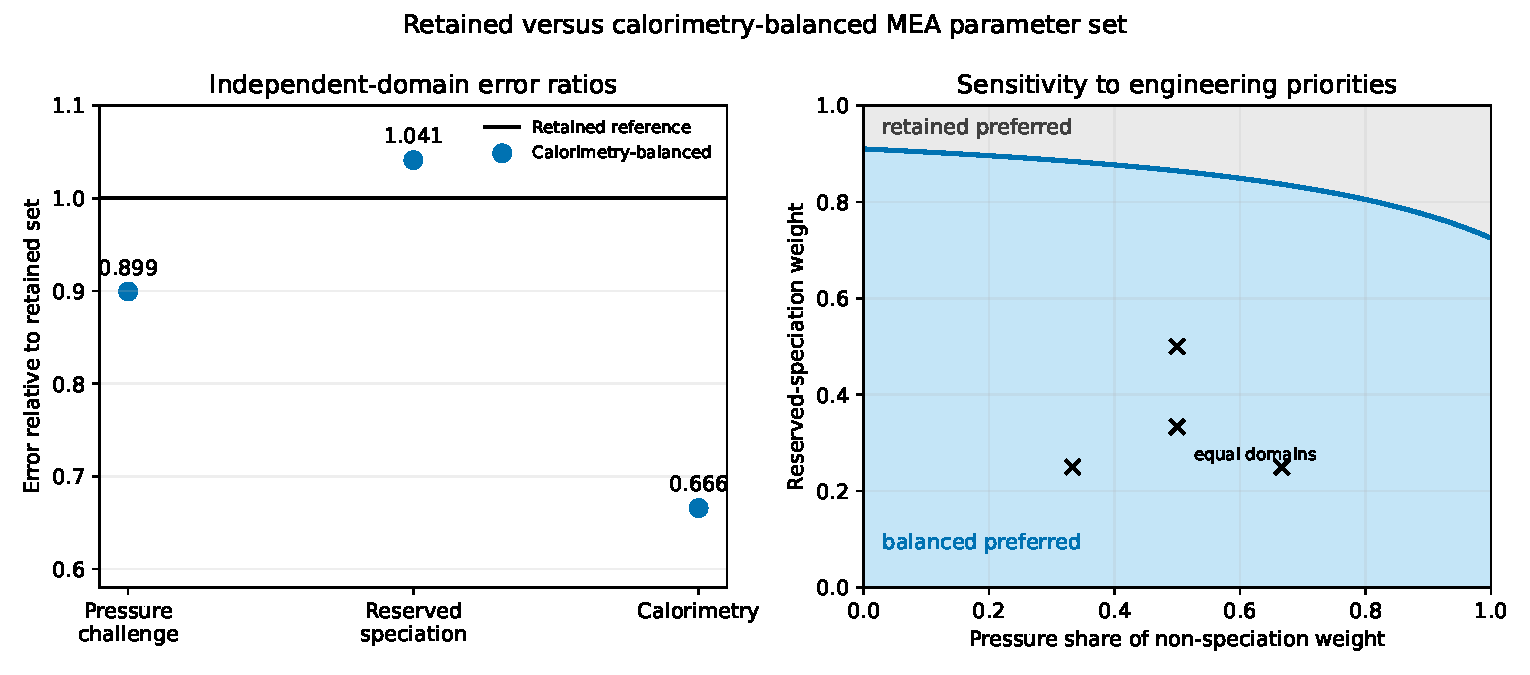
\includegraphics[width=\textwidth]{analyses/phase3/ionic_epcsaft_regression/born_permittivity_sensitivity/figures/independent_evidence_comparison.pdf}
\caption{Independent-domain error ratios and sensitivity of the preferred
parameter set to engineering priorities. The exact plotted values are retained
beside the figure.}
\end{figure}

\subsection{Interpretation and limitations}

The calorimetry-balanced candidate has the lower diagnostic score under equal
weighting and under each tested single-domain-emphasis profile. The retained
set remains preferable only for a decision dominated almost entirely by
former-reserved speciation. This ranking does not support parameter adoption or
absorber-model transfer.

The comparison does not establish statistical selection. Speciation and
calorimetry observations include correlated rows, and full covariance matrices
are unavailable. The calorimetry observable is a Gibbs--Helmholtz diagnostic
that neglects the pressure--volume correction and represents an average
313.15--353.15 K temperature derivative. Exact inputs and results are retained
under
\texttt{results/independent\_evidence\_comparison/} in the Born-permittivity
analysis directory.
